\chapter{Introduction}
\label{chapter:introduction}

One of the main goals in computer graphics is realistic rendering. 
Even though computer graphics is constantly improving, we are still quite away from reality because material representation in a traditional way lack important realistic properties. 
A 2-D texture in conjunction with a shading model is a conventional way to represent material appearance in rendering.
On the other side, real-world materials surfaces consist of surface meso-structures, i.e. intermediate in size local geometric details.
Meso-structures are responsible for fine-scale shadows, self-occlusions, inter-reflection, subsurface scattering and specularities.
Also, reflectance and the look of the real-world materials can drastically change when camera and light direction vary.

One of the possible solution to represent such material's attributes is to use sophisticated light functions, for instance a Bidirectional Texture Function (BTF). 
 A BTF is a 6-dimensional function that depends on camera and light directions as well as on spatial texture coordinates. 
The BTF conceptually extends traditional 2-D texture by the dependence on light and camera directions.
This function is usually acquired as a data-set of thousands images that cover discrete light and camera directions.
Due to enormous size of such data direct rendering even on the modern hardware without any compression is impractical.
Fortunately, there exist many techniques to deal with huge size of BTF, i.e. compression methods that were developed for BTF.


In this thesis, we introduce \emph{WebGL}-based rendering for BTF over the Internet.
Till now lots of emphasize were done for rendering 3-D objects in a web-browser using \emph{WebGL}-based technique.
Computer graphics in a web-browser is becoming popular for games and visualization.
The reason of such popularity is that the user does not need to install any additional applications and WebGl-based rendering is cross-platform technology, which require only compatible browser.
Therefore, it is very handy for the user.

Even though 3-D graphics for web-browsers is gaining popularity, BTF was rarely implemented for \emph{WebGL} standard, due to its huge size and overall computational effort to render.
This usually includes: decompression of BTF, computation  and interpolation for camera and light directions.
Such demanding computational effort may be time consuming, especially for low-budget devices such as mobile-devices, old laptops and PCs.

The other problem which arise when rendering BTF over the Internet is the transmission of the data.
Before WebGl can start rendering on the client side, the transmission of the data must be finished beforehand.
Even to transfer a compressed BTF data can be time consuming for the user. 
The compressed BTF can be around few megabytes of size, therefore it would it take some time to transfer the data.
Consider the worst-case scenario, i.e. an average internet connection of a common user around 5 Mbit/s and a compressed BTF data size around 20 Mb.
This will take around 30sec to download. Even though, it sounds as not a big of problem, but any user would like to see the result as quick as possible.
One possible solution to this problem is a streaming of the data. 
With the streaming technology the user may be able to see the first preview of the 3-D object just in a few seconds.
We introduce  \emph{Web-Sockets} technique, which is supported by most of the contemporary browsers.
With \emph{Web-Sockets}  the  full-duplex communication is available for the server and the client, which is faster than traditional HTTP-based methods. 
This promises fast and reliable solution for real-time performance in \emph{WebGL}-based application.

In summary main contributions of this paper are:

\begin{itemize}
 \item PCA compression on subsets of BTF
 \item improvement of PCA compression error by scaling the resulted parameters
 \item linear interpolation for camera and light directions using barycentric coordinates
 \item BTF streaming using \emph{Web-Sockets} technology
 \item prioritized streaming order of BTF parameters, which let the progressive improvement of the rendering quality
 \item introduced ambient light term which depends on the light direction, which makes the object look less artificial
 \item implemented \emph{WebGL}-based demo web-application and \emph{Web-Sockets} server
\end{itemize}


\section{Related Work}
\label{section:related_work}


 Lately 3D content started to gain popularity in context of web-based applications.
 New standards for 3D graphics in context of HTML domain are evolving, for instance such as XML3D \cite{xml3d}.
 That means that demand for realistic rendering in web-based context will grow.
 Such 3D web-based applications can be aimed for arbitrary websites.
 Any commercial website could represent their product as a 3D content for marketing purposes, so the future customers could examine the desired product fully in 3D.
 Thus, realistic rendering would be highly desirable to make the best impression on the customer.
 
 Until now previous works that used BTF compression for realistic rendering were primarily intended  for offline application, i.e. standalone application.
However, such approach may be not suitable in context of web-based application, due to the data transfer between the server and the client, which can delay the rendering for certain time.
  Schwartz \emph{et. al.} \cite{webglbtfstreaming} presented a work in which compressed BTF data is streamed from the server to the client.
 The streaming over the Internet is done by means of HTTP streaming, i.e. the web-application requests the data in small chunks.
 With each new chunk of the BTF data the rendering quality of the 3D object is progressively enhanced.
 We on the other hand, deploy \emph{Web-Sockets} technology, which can improve application performance compared to HTPP streaming, by reducing the network latency and an option to stream the data in a binary form.

 
 Up-to-date existing BTF compression methods are reviewed by Haindl \emph{et. al.} \cite{haindl, haindl_visual}.
 Depending on the intended application, a trade-off has to be made between a rendering quality and a compression rate.
Our compression method is related to PCA RF (Principal Component Analysis Reflectance Field) method, which was introduced by Sattler \emph{et. al.} \cite{star2004}.
This method allows for real-time performance with realistic rendering quality. 
Sattler perform PCA on each of $n$ camera directions separately. We on the other hand, perform PCA on $k$ neighbour camera directions at once.
In Haindl's review \cite{haindl} PCA based methods achieve better or at least not worse reconstruction quality results than most others methods.
Compression rates of PCA methods are mild compared to other methods, however those methods which produce better compression rates have worse quality than PCA based methods.
To overcome the problem of mild compression rates in web-based application, we introduce streaming with \emph{Web-Sockets}, which allows to start rendering just in a few seconds.
During the streaming the rendering quality improves.


\section{Outline}
\label{section:outline}

\begin{figure}[h]
 \centering
 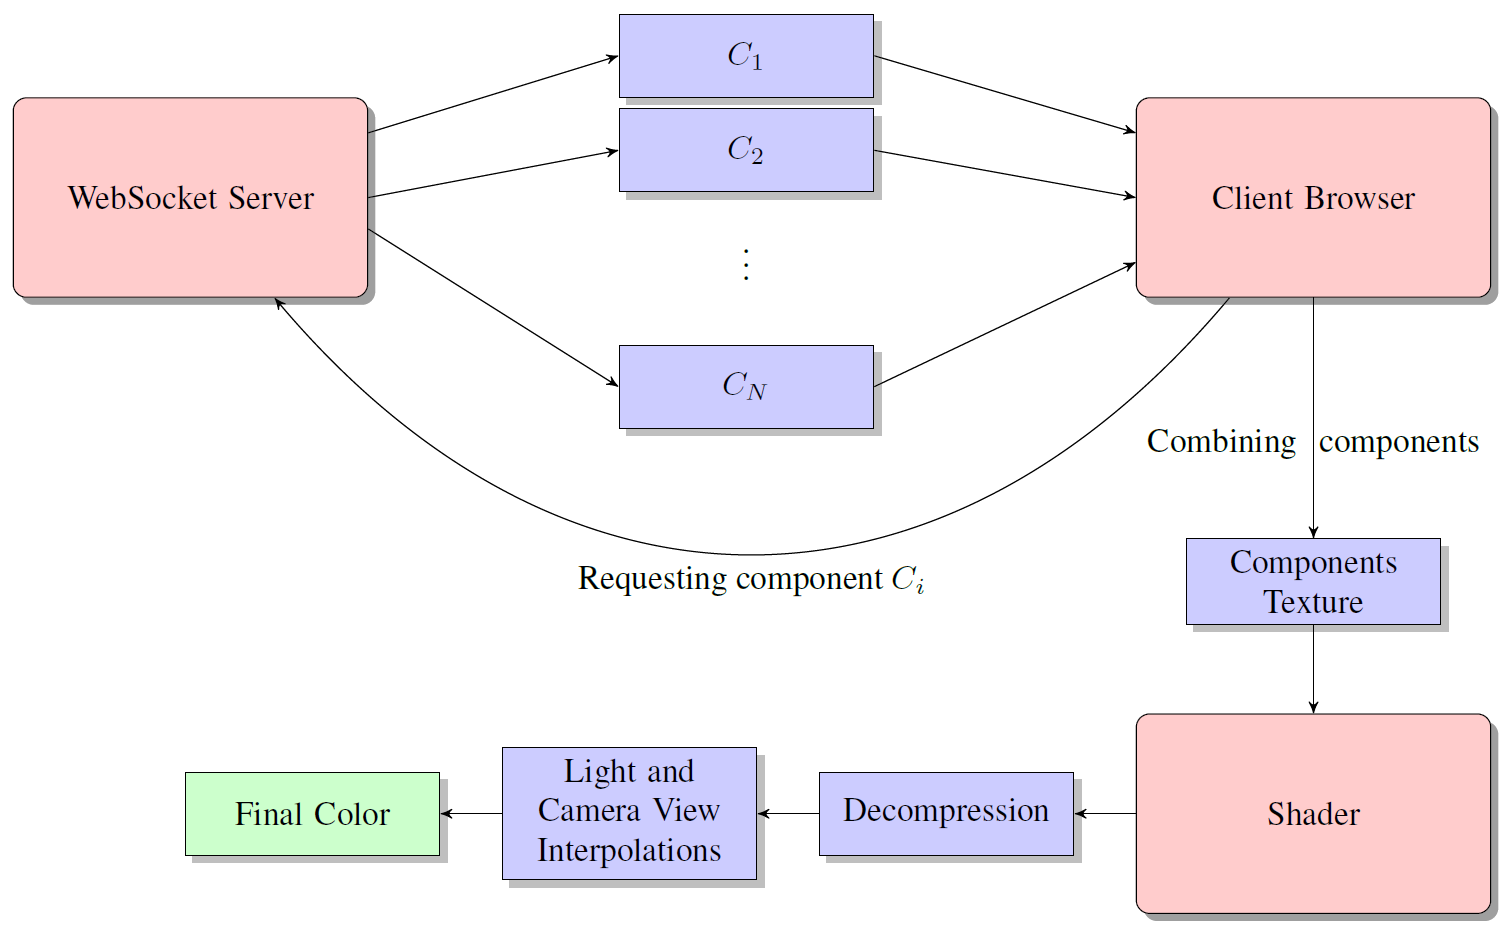
\includegraphics[width=1.0\textwidth]{figures/overview}
 \caption[Model Overview ] {
 	{\bf Model Overview}

	
	}
 \label{fig:overview}
\end{figure}



